\documentclass{anstrans}
%%%%%%%%%%%%%%%%%%%%%%%%%%%%%%%%%%%
\title{Improved Quasi-Static Method with Step Doubling Time Adaptation}
\author{Zachary M. Prince, Jean C. Ragusa}

\institute{
Department of Nuclear Engineering, Texas A\&M University, College Station, TX
}

\email{zachmprince@tamu.edu \and jean.ragusa@tamu.edu}

% Optional disclaimer: remove this command to hide
%\disclaimer{Notice: this manuscript is a work of fiction. Any resemblance to actual articles, living or dead, is purely coincidental.}

%%%% packages and definitions (optional)
\usepackage{color} % allows inclusion of graphics
\usepackage{graphicx} % allows inclusion of graphics
\usepackage{booktabs} % nice rules (thick lines) for tables
\usepackage{microtype} % improves typography for PDF
\usepackage{subcaption}

\newcommand{\SN}{S$_N$}
\renewcommand{\vec}[1]{\bm{#1}} %vector is bold italic
\newcommand{\vd}{\bm{\cdot}} % slightly bold vector dot
\newcommand{\ud}{\mathop{}\!\mathrm{d}} % upright derivative symbol
%  new definitions
\newcommand{\bs}[1]{\mathbf{#1}}
\renewcommand{\div}{\bs{\nabla}\! \cdot \!}
\newcommand{\grad}{\bs{\nabla}}
% extra space
\newcommand{\qq}{\quad\quad}
% common reference commands
\newcommand{\eqt}[1]{Eq.~(\ref{#1})}                     % equation
\newcommand{\fig}[1]{Fig.~\ref{#1}}                      % figure
\newcommand{\tbl}[1]{Table~\ref{#1}}                     % table
\newcommand{\sct}[1]{Section~\ref{#1}}                   % section
\newcommand{\app}[1]{Appendix~\ref{#1}}                   % appendix

\newcommand{\keff}{k_\textit{eff}}

\newcommand{\be}{\begin{equation}}
\newcommand{\ee}{\end{equation}}
\newcommand{\vn}{\vec{n}}
\newcommand{\vel}{\vec{\mathrm{v}}}
\newcommand{\adj}{\Phi^\dagger_0}
\newcommand{\tcr}[1]{\textcolor{red}{#1}}
\newcommand{\norm}[1]{\left\lVert#1\right\rVert_{L^2}}


\begin{document}
%%%%%%%%%%%%%%%%%%%%%%%%%%%%%%%%%%%%%%%%%%%%%%%%%%%%%%%%%%%%%%%%%%%%%%%%%%%%%%%%

\section{Introduction}
The imminent restart of the Transient Reactor Testing Facility (TREAT) at Idaho National Laboratory (INL) has brought significant attention to the development of transient reactor modeling.  TREAT was designed to subject fuels and other reactor components to various degrees of neutron pulses, from minor transients to accident scenario.  Inherently, this task requires predicting pulse responses due to various control rod movements; which is a complicated endeavor.  Originally, this was done using an iterative process of rod movements and measuring the resulting response.  With the advances in computer modeling, the current goal, preceding the restart, is to use simulation to characterize responses before experiments take place.  However, neutron transient modeling is extremely computationally expensive due to the required implicit time-stepping.  Therefore, methods that mitigate computation time, with minimal detriment to accuracy, are highly desired.  This paper will describe the improved quasi-static method (IQS), which hopes to decrease computation time significantly from traditional "brute force" transient methods.

IQS is a spatial kinetics method that involves factorizing the flux solution into time-dependent amplitude and space- and time-dependent shape \cite{Ott_1966,Dulla2008}.  The impetus of the method is the assumption that shape is weakly time-dependent, so expensive space-dependent evaluations are only required on large time steps.  While inexpensive amplitude evaluations are performed on much smaller time steps to retain accuracy.  IQS has been tested extensively on kinetics benchmarks with constant time steps.  However, to test it's viability for TREAT simulations, evaluating IQS's performance with time adaptation is required.  The rest of this paper will briefly describe the derivation of IQS, the time adaptation technique used, and results from a kinetic benchmarks.

%%%%%%%%%%%%%%%%%%%%%%%%%%%%%%%%%%%%%%%%%%%%%%%%%%%%%%%%%%%%%%%%%%%%%%%%%%%%%%%%
\section{Theory}
In this Section, we recall the equation for the IQS method, starting from the standard multi-group transport equations with delayed neutron precursors in operator form:

\be
\frac{1}{v^g}\frac{\partial \Psi^g}{\partial t} = \sum_{g'=1}^G \left(H^{g'\to g} + P_p^{g' \to g} \right) \Psi^{g'} - L^g\Psi^g + S_{d}^g
\label{eq:flux}
\ee 
\be
\frac{dC_i}{dt} = \sum_{g=1}^G P_{d,i}^g \Psi^{g} - \lambda_i C_i \ , \quad 1 \le i \le I 
\label{eq:precursor}
\ee

Factorization is an important step in the derivation of the IQS method. The factorization approach leads to a decomposition of the multigroup flux into the product of a time-dependent amplitude ($p$) and a space-/time-dependent multigroup shape ($\psi$):
\be
\Psi^g(\vec{r},\Omega,t)=p(t)\psi^g(\vec{r},\Omega,t)
\ee
To obtain the amplitude equations, the multigroup equations are multiplied by a weighting function, typically the initial adjoint flux ($\phi^*$), and then integrated over phase-space.  For brevity, the inner product over space will be represented with parenthetical notation ($\left(\Psi^{*g},f^g\right) = \int_{4\pi}\int_D \Psi^{*g}(\vec{r},\vec{\Omega})f^g(\vec{r},\vec{\Omega})d^3r d^2\Omega
$).  In order to impose uniqueness of the factorization, one requires $\sum_{g=1}^G\left(\Psi^{*g},\frac{1}{v^g}\psi^g\right)$ to be constant.  And after some manipulation, the standard point reactor kinetics equations (PRKE) for the amplitude solution are obtained:
\be
\frac{dp}{dt}=\left[\frac{\rho-\bar{\beta}}{\Lambda}\right]p+\sum_{i=1}^I\bar{\lambda}_i\xi_i
\ee
\be
\frac{d\xi_i}{dt}=\frac{\bar{\beta}_i}{\Lambda}p-\bar{\lambda}_i\xi_i \quad 1 \le i \le I 
\ee
Where the functional coefficients are calculated using the space-/time-dependent shape function as follows:
%\begin{align}
%\frac{\rho-\bar{\beta}}{\Lambda}=&\Bigg[\sum_{g=1}^G \bigg(\phi^{*g},\frac{\chi_p^g}{k_{eff}}(1-\beta)\sum_{g'=1}^G \nu^{g'} \Sigma_f^{g'}\varphi^{g'} + \sum_{g'\neq g}^G\Sigma_s^{g'\to g} \varphi^{g'} \nonumber \\
%& -\left( -\div D^g \grad  + \Sigma_r^g \right)\varphi^g \bigg)\Bigg] \times \Bigg[\sum_{g=1}^G\left(\phi^{*g},\frac{1}{v^g}\varphi^g\right)\Bigg]^{-1}
%\label{eq:rmb}
%\end{align}
%\be
%\frac{\bar{\beta}}{\Lambda}=\sum_{i=1}^I\frac{\bar{\beta}_i}{\Lambda}=\sum_{i=1}^I\frac{1}{k_{eff}}\frac{\sum_{g=1}^G(\phi^{*g}, \chi_{d,i}^g\beta_i\sum_{g'=1}^G\nu^{g'} \Sigma_f^{g' }\varphi^{g'})}{\sum_{g=1}^G\left(\phi^{*g},\frac{1}{v^g}\varphi^g\right)}
%\label{eq:b}
%\ee
%\be
%\bar{\lambda}_i=\frac{\sum_{g=1}^G(\phi^{*g},\chi_{d,i}^g\lambda_i C_i)}{\sum_{g=1}^G(\phi^{*g},\chi_{d,i}^gC_i)}
%\label{eq:l}
%\ee
\be
\frac{\rho-\bar{\beta}}{\Lambda}=\frac{ \sum_{g=1}^G\left(\Psi^{*g},\sum_{g'}(H^{g' \to g}+P_p^{g' \to g}-L^{g'}\delta_{g'g})\psi^{g'}\right)}{\sum_{g=1}^G\left(\Psi^{*g},\frac{1}{v^g}\psi^g\right)}
\label{eq:rmb}
\ee
\be
\frac{\bar{\beta}}{\Lambda}=\sum_{i=1}^I\frac{\bar{\beta}_i}{\Lambda}=\sum_{i=1}^I\frac{\sum_{g=1}^G(\Psi^{*g}, P_{d,i}^g \psi^g)}{\sum_{g=1}^G\left(\Psi^{*g},\frac{1}{v^g}\psi^g\right)}
\ee
\be
\bar{\lambda}_i=\frac{\sum_{g=1}^G(\Psi^{*g},\chi_{d,i}^g\lambda_i C_i)}{\sum_{g=1}^G\left(\Psi^{*g},\frac{1}{v^g}\psi^g\right)}
\label{eq:l}
\ee

%%%%%%%%%%%%%%%%%%%%%%%%%%%%%%%%%%%%%%%%%%%%%%%%%%%%%%%%%%%%%%%%%%%%%%%%%%%%%%%%
\subsection{IQS Predictor-Corrector (IQS P-C)}

This version of IQS first solves the flux diffusion (represented by Equations \ref{eq:flux} and \ref{eq:precursor}) to get a predicted flux.  The predicted flux at this step is then converted to shape by rescaling as follows:
\be
\psi^g_{n+1} = \underbrace{\Psi^g_{n+1}}_{\text{predicted}} \frac{K_0}{K_{n+1}}
\label{eq:rescale}
\ee
Where:
\be
K_{n+1} =\sum_{g=1}^G\left(\Psi^{*g},\frac{1}{v^g}\Psi^g_{n+1}\right)
\ee
\be
K_{0} =\sum_{g=1}^G\left(\Psi^{*g},\frac{1}{v^g}\psi^g_{n+1}\right)=\sum_{g=1}^G\left(\Psi^{*g},\frac{1}{v^g}\Psi^g_{0}\right)
\ee

The PRKE parameters are then computed with this shape using Equations \ref{eq:rmb} - \ref{eq:l} and interpolated over the macro step, then the PRKE is evaluated.  With the newly computed amplitude, the shape is rescaled and the corrected flux is evaluated:
\be
\underbrace{\Psi^g_{n+1}}_{\text{corrected}} = p_{n+1} \times \psi^g_{n+1}
\ee

%%%%%%%%%%%%%%%%%%%%%%%%%%%%%%%%%%%%%%%%%%%%%%%%%%%%%%%%%%%%%%%%%%%%%%%%%%%%%%%%
\subsection{Time Adaptation}

The time adaptation used for quantifying IQS's ability is step doubling.  The step doubling technique involves estimating the local truncation error for a certain time step by taking the difference between a solution with one full step and a solution with two half steps.  If the step is small enough, the error will be smaller than a user driven tolerance and the magnitude of the next step will be calculated based on the error.  If the step is too large, the step will be repeated with a smaller step calculated with the resulting error.  The error of the time step is approximated by Equation \ref{eq:edt2}, where $\Psi^g_{\Delta t}$ and $\Psi^g_{\Delta t/2}$ are the solutions with the full step and half step, respectively.  If $e_n > e_{max}$ the time step is repeated; if $e_n < e_{max}$ the system moves to the next time step.  The next $\Delta t$ is calculated using Equation \ref{eq:dt2}, where $\mu$ is the convergence order of the time integration scheme being used.  $e_{max}$ and $e_{tol}$ are user defined parameters; $e_{max}$ is usually less than $e_{tol}$ to better guarantee that the calculated $\Delta t_{new}$ will pass the error criteria so time steps won't be repeated.

\be
e_n = \frac{\norm{\sum_{g=1}^G\int_{4\pi}\Psi^g_{\Delta t/2} d^2\Omega - \sum_{g=1}^G\int_{4\pi}\Psi^g_{\Delta t} d^2\Omega}}{\text{max}\left(\norm{\sum_{g=1}^G\int_{4\pi}\Psi^g_{\Delta t/2} d^2\Omega},\norm{\sum_{g=1}^G \int_{4\pi}\Psi^g_{\Delta t} d^2\Omega}\right)}
\label{eq:edt2}
\ee
\be
\Delta t_{new} = \Delta t \left(\frac{e_{tol}}{e_n}\right)^{\frac{1}{\mu+1}}
\label{eq:dt2}
\ee 

%%%%%%%%%%%%%%%%%%%%%%%%%%%%%%%%%%%%%%%%%%%%%%%%%%%%%%%%%%%%%%%%%%%%%%%%%%%%%%%%
\section{Results and Analysis}
This section describes results of the TWIGL benchmark that tests the IQS implementation and shows its effectiveness on computation speed and accuracy.  The benchmark was solved with regular diffusion (brute force) and IQS P-C with backward-Euler time discretization.  The performance for each method are represented by the number of macro time steps and solves with step doubling time adaptation.

%%%%%%%%%%%%%%%%%%%%%%%%%%%%%%%%%%%%%%%%%%%%%%%%%%%%%%%%%%%%%%%%%%%%%%%%%%%%%%%%
\subsection{TWIGL Benchmark}

This benchmark problem originates from the Argonne National Lab Benchmark Problem Book (8-A1-1) \cite{ANL_BPB}.  It is a 2D, 2-group reactor core model with no reflector region, the geometry, material properties, and transient perturbation can be seen in \cite{TWIGL_benchmark}. Figure \ref{fig:TWIGL_power} shows the IQS  solution as compared with the Brute Force solution with minimal time steps.  Table \ref{tab:TWIGLdt2} shows the results for time adaptation.  The results show that IQS performs exceptionally well compared to brute force for this highly transient example.

%\begin{figure}[!htbp]
%\begin{center}
%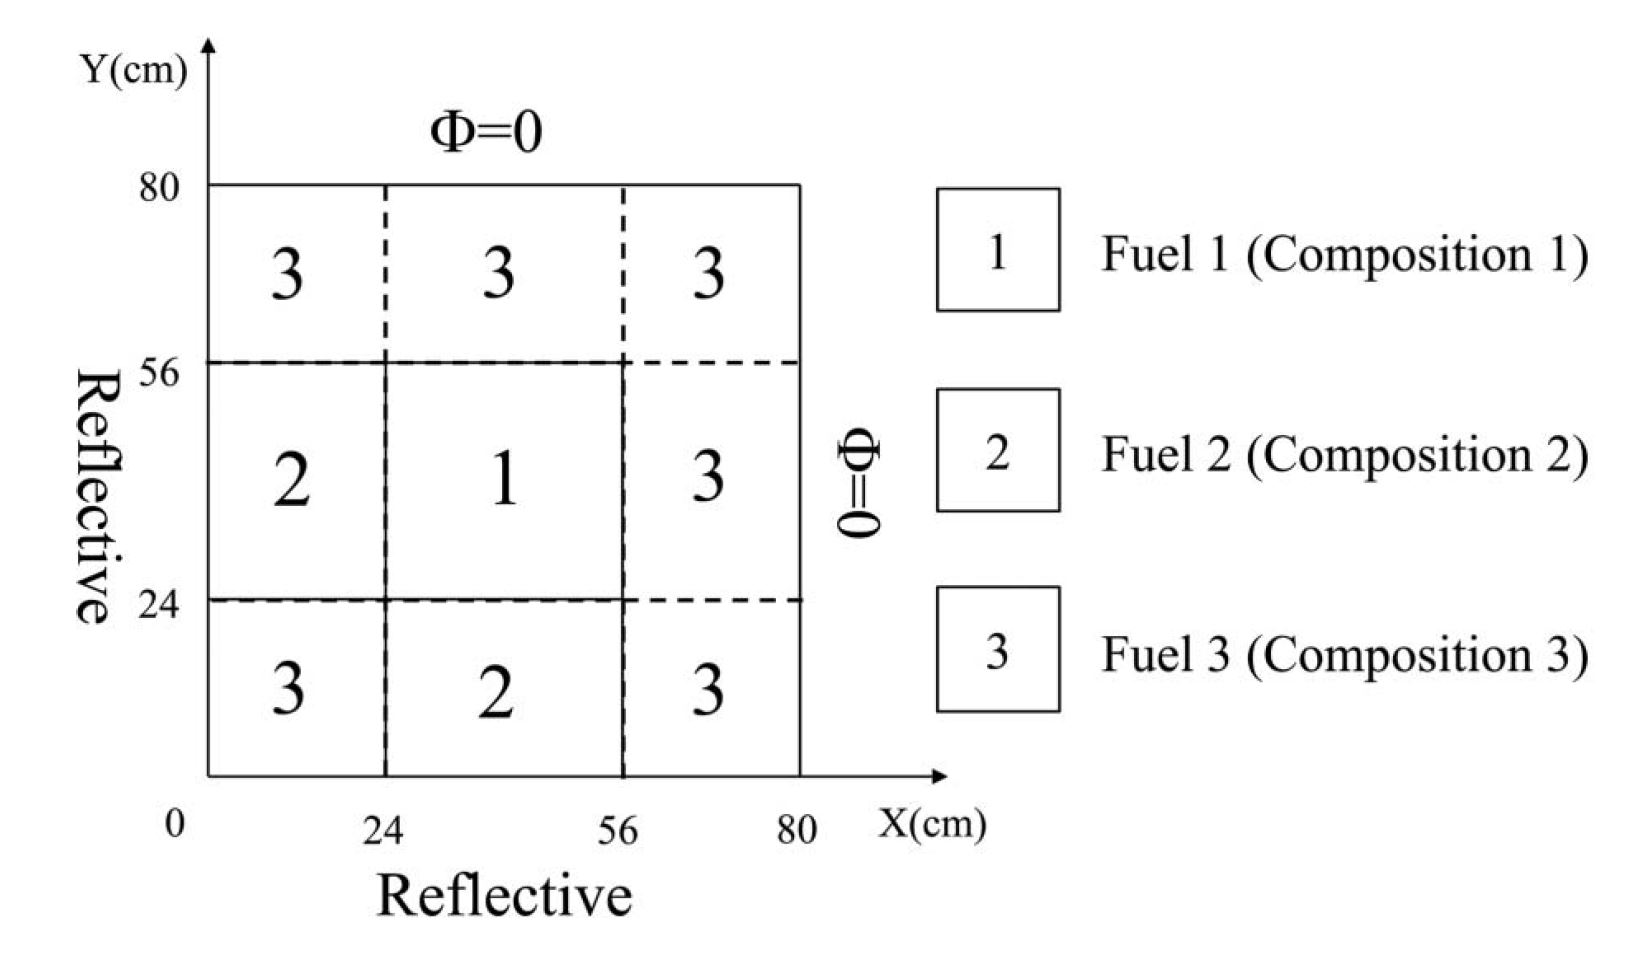
\includegraphics[width=0.45\textwidth]{TWIGL_regions.jpg}
%\caption{TWIGL benchmark problem description}
%\label{fig:TWIGL_reg}
%\end{center}
%\end{figure}
%
%\begin{table}[!htbp]
%\begin{center}
%\resizebox{0.45\textwidth}{!}{
%\begin{tabular}{llllllll}
%\hline
%  &  &  &  &  &  &  \multicolumn{2}{c}{$\underline{\Sigma_s (cm^{-1})} $} \\
%Material & Group & $D (cm)$ & $\Sigma_a (cm^{-1})$ & $\nu\Sigma_f (cm^{-1})$ & $\chi$ & $g \rightarrow 1$ & $g \rightarrow 2$ \\
%\hline
%1 & 1 & 1.4 & 0.010 & 0.007 & 1.0 & 0.0 & 0.01 \\
%  & 2 & 0.4 & 0.150 & 0.200 & 0.0 & 0.0 & 0.00  \\
%2 & 1 & 1.4 & 0.010 & 0.007 & 1.0 & 0.0 & 0.01  \\
%  & 2 & 0.4 & 0.150 & 0.200 & 0.0 & 0.0 & 0.00  \\
%3 & 1 & 1.3 & 0.008 & 0.003 & 1.0 & 0.0 & 0.01  \\
%  & 2 & 0.5 & 0.050 & 0.060 & 0.0 & 0.0 & 0.00  \\
%\hline
%  & $\nu$ & $v_1 (cm/s)$ & $v_2 (cm/s)$ & $\beta$ & $\lambda (1/s)$ &   &   \\
%\hline
%  & 2.43 & 1.0E7 & 2.0E5 & 0.0075 & 0.08 &   &   \\
%\hline
% \multicolumn{8}{l}{Material 1 ramp perturbation:} \\
%\multicolumn{8}{l}{$\Sigma_{a,2}(t)=\Sigma_{a,2}(0) \times (1-0.11667t) \quad t \leq 0.2 s$} \\
%\multicolumn{8}{l}{$\Sigma_{a,2}(t)=\Sigma_{a,2}(0) \times (0.97666t) \quad t > 0.2 s$} \normalsize
%\end{tabular}}
%\end{center}
%\caption{TWIGL benchmark material properties and slope perturbation}
%\label{tab:TWIGL_mat}
%\end{table}

\begin{figure}[!htbp]
\centering
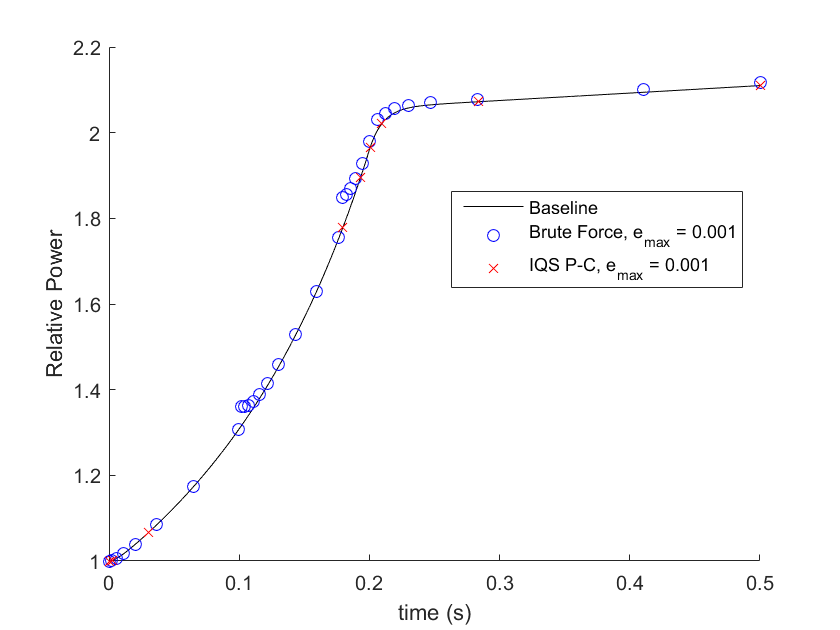
\includegraphics[width=0.45\textwidth]{figures/TWIGL_power_plot.png}
\caption{Power level comarison of TWIGL benchmark between IQS and Brute Force using $e_{max} = 0.001$}
\label{fig:TWIGL_power}
\end{figure}

\begin{table}[!htbp]
\begin{center}
\resizebox{0.45\textwidth}{!}{
\begin{tabular}{|l|l|l|l|l|l|l|l|}
\hline
  &  & \multicolumn{3}{|c|}{Brute Force} & \multicolumn{3}{|c|}{IQS P-C} \\
\hline
Test & $e_{max}$ & Error & Steps & Solves & Error & Steps & Solves \\
\hline
1 &	0.05    &	0.00012677 &	9    &	29   &	0.03380433 &	4  &	9   \\
2 &	0.01    &	3.5555e-05 &	11   &	35   &	0.00263068 &	5  &	12  \\
3 &	0.005   &	4.0364e-05 &	11   &	31   &	0.00160486 &	6  &	21  \\
4 &	0.001   &	0.00294822 &	33   &	122  &	1.7527e-05 &	10 &	35  \\
5 &	0.0005  &	0.00099778 &	39   &	131  &	1.4185e-05 &	16 &	74  \\
6 &	0.0001  &	0.00019510 &	78   &	236  &	6.2903e-06 &	19 &	78  \\
7 &	5.0e-05 &	0.00018372 &	112  &	342  &	1.5247e-06 &	24 &	92  \\
8 &	1.0e-05 &	8.0564e-05 &	263  &	794  &	9.8321e-07 &	48 &	210 \\
\hline

\end{tabular}}
\end{center}
\caption{TWIGL step doubling results}
\label{tab:TWIGLdt2}
\end{table}

%%%%%%%%%%%%%%%%%%%%%%%%%%%%%%%%%%%%%%%%%%%%%%%%%%%%%%%%%%%%%%%%%%%%%%%%%%%%%%%%
%\subsection{LRA Benchmark}
%
%The LRA benchmark is a two-dimensional, two-group neutron diffusion problem with adiabatic heat-up and Doppler feedback in thermal reactor \cite{BPB}.  It is a super prompt-critical transient.  To have better understanding on the cross sections given later, we present the equations here:
%\begin{align}
%-\frac{1}{v_1} \frac{\partial \phi_1}{\partial t} &= -\grad D_1 \grad\phi_1 + (\Sigma_{a,1} + \Sigma_{s, 1\rightarrow 2})\phi_1 \nonumber \\
%&- \nu(1-\beta)S_f  - \sum_{i=1}^2 \lambda_i C_i, \\
%-\frac{1}{v_2} \frac{\partial \phi_2}{\partial t} &= -\grad D_2 \grad\phi_1 + \Sigma_{a,2}\phi_2 - \Sigma_{s, 1\rightarrow 2}\phi_1, \\
%S_f &= \sum_{g=1}^2 \Sigma_{f,g} \phi_g, \\
%\frac{\partial C_i}{\partial t} &= \nu\beta_i f - \lambda_i C_i, \quad i=1,2, \\
%\frac{\partial T}{\partial t} &= \alpha f, \label{eq:lra-temp} \\
%\Sigma_{a,1} &= \Sigma_{a,1}(\vec{r}, t=0) \left[1+\gamma\left(\sqrt{T} - \sqrt{T_0}\right)\right], \\
%P &= \kappa S_f,
%\end{align}
%where $\phi_1$, $\phi_2$ are the fast and thermal fluxes; $v_1, v_2$ are the averaged neutron velocities; $\Sigma_{a,1}, \Sigma_{a,2}$ are the absorption cross sections; $\Sigma_{s,1\rightarrow 2}$ is the fast-to-thermal scattering cross section; $\Sigma_{f,1}, \Sigma_{f,2}$ are the fission cross sections; $\nu$ is the averaged number of neutrons emitted per fission; $\beta_1, \beta_2$ are the delayed neutron precursor fractions and $\beta=\beta_1 + \beta_2$; $C_1, C_2$ are the delayed neutron precursor concentrations; $\lambda_1, \lambda_2$ are the decay constants of the delayed neutron precursors; $S_6f$ is the fission reaction rate; $P$ is the power density; $T$ is the temperature; $\kappa$ is the averaged power released per fission; $\alpha$ is the combination of $\kappa$ and the specific heat capacity; $\gamma$ is the Doppler feedback coefficient; $T_0=T(\vec{r}, t=0)$.
%The two-group diffusion equation are solved with zero flux boundary conditions on external surfaces, reflecting conditions at symmetry boundaries and steady state initial conditions which are obtained by solving
%\begin{align}
%-\grad D_1 \grad\phi_1 + (\Sigma_{a,1} + \Sigma_{s, 1\rightarrow 2})\phi_1 &= \frac{1}{k}\sum_{g=1}^2 \nu\Sigma_{f,g}\phi_g, \\
%-\grad D_2 \grad\phi_1 + \Sigma_{a,2}\phi_2 =& \Sigma_{s, 1\rightarrow 2}\phi_1
%\end{align}
%The eigenvalue $k$ is used to modify the fission cross section for the transient simulations with $\frac{1}{k}\Sigma_{f,g}, g=1,2$.  The initial flux distribution shall be normalized such that the averaged power density
%\begin{align}
%\bar{P} \equiv \frac{\int_{V_{core}} P(\vec{r}, t=0) d\vec{r}}{\int_{V_{core}} d\vec{r}},
%\end{align}
%where $V_{core}$ is the core region with fuels, is equal to $10^{-6} W\cdot cm^{-3}$.
%The initial precursor concentrations are in equilibrium with the initial critical flux distribution.\\
%
%The geometry is illustrated in~\fig{fig:lra-geometry}.\\
%\begin{figure}[!htbp]
%\centering
%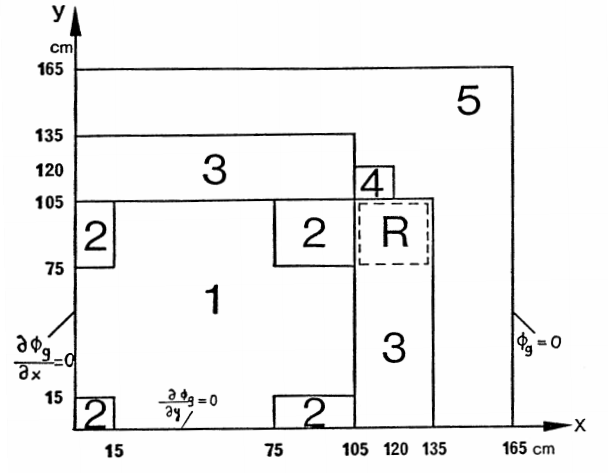
\includegraphics[width=0.8\linewidth]{lra.png}
%\caption{LRA benchmark geometry with region assignment.}
%\label{fig:lra-geometry}
%\end{figure}
%
%Initial two-group constants are presented in~\tbl{tab:lra-xs}.
%$\nu$ is equal to 2.43.
%Axial bulking $B^2 = 10^{-4}$ is applied for both energy groups.
%Delayed neutron data are presented in~\tbl{tab:lra-dnp}.
%All fuel materials have the same delayed neutron data.
%Some scalar data are listed in~\tbl{tab:lra-scalar}.\\
%\begin{table}[!htbp]
%    \centering
%    \resizebox{0.5\textwidth}{!}{
%      \begin{tabular}{|c|c|c|c|l|l|l|l|l|}
%      \hline
%             &                 & Group   & $D_g$      & $\Sigma_{a,g}$ & $\nu\Sigma_{f,g}$ & $\Sigma_{s,1\rightarrow 2}$ & $\chi_g$ & $v_g$              \\
%      Region & Material        &       g & (cm)       &  ($cm^{-1}$)   &  ($cm^{-1}$)      &  ($cm^{-1}$)                &          & ($cm\cdot s^{-1}$) \\
%      \hline
%      1      & Fuel 1 with rod & 1       & 1.255      & 0.008252       & 0.004602          &                             & 1        & $3.0\times10^7$    \\
%             &                 & 2       & 0.211      & 0.1003         & 0.1091            & 0.02533                     & 0        & $3.0\times10^5$    \\
%      \hline
%      2      & Fuel 1 without rod & 1    & 1.268      & 0.007181       & 0.004609          &                             & 1        & $3.0\times10^7$    \\
%             &                    & 2    & 0.1902     & 0.07047        & 0.08675           & 0.02767                     & 0        & $3.0\times10^5$    \\
%      \hline
%      3      & Fuel 2 with rod & 1       & 1.259      & 0.008002       & 0.004663          &                             & 1        & $3.0\times10^7$    \\
%             &                 & 2       & 0.2091     & 0.08344        & 0.1021            & 0.02617                     & 0        & $3.0\times10^5$    \\
%      \hline
%      4      & Fuel 2 without rod & 1    & 1.259      & 0.008002       & 0.004663          &                             & 1        & $3.0\times10^7$    \\
%             &                    & 2    & 0.2091     & 0.073324       & 0.1021            & 0.02617                     & 0        & $3.0\times10^5$    \\
%      \hline
%      5      & Reflector        & 1      & 1.257      & 0.0006034      & -                 &                             & -        & $3.0\times10^7$    \\
%             &                  & 2      & 0.1592     & 0.01911        & -                 & 0.04754                     & -        & $3.0\times10^5$    \\
%      \hline
%      \end{tabular}}
%    \caption{LRA benchmark initial two-group constants.\label{tab:lra-xs}}
%\end{table}
%
%\begin{table}[!htbp]
%    \centering
%      \begin{tabular}{|c|l|l|l|l|}
%      \hline
%      Group i & $\beta_i$ & $\lambda_i$ ($s^{-1}$) & $\chi_{d,i,1}$ & $\chi_{d,i,2}$ \\
%      \hline
%      1       & 0.0054    & 0.0654  & 1 & 0 \\
%      2       & 0.001087  & 1.35    & 1 & 0 \\
%      \hline
%      \end{tabular}
%    \caption{LRA benchmark delayed neutron data.\label{tab:lra-dnp}}
%\end{table}
%
%\begin{table}[!htbp]
%    \centering
%    \resizebox{0.5\textwidth}{!}{
%      \begin{tabular}{|l|c|l|}
%      \hline
%      Meaning & Notation & value \\
%      \hline
%      Axial buckling for both energy groups & $B_g^2$  & $10^{-4}$ ($cm^{-2}$)\\
%      Mean number of neutrons per fission   & $\nu$    & 2.43 \\
%      Conversion factor                     & $\alpha$ & $3.83\times 10^{-11}$ ($K\cdot cm^{3}$) \\
%      Feedback constant                     & $\gamma$ & $3.034\times 10^{-3}$ ($K^{1/2}$) \\
%      Energy released per fission           & $\kappa$ & $3.204\times 10^{-11} $ ($J/fission$) \\
%      Initial and reference temperature     & $T_0$    & 300 (K) \\
%      Active core volume                    & $V_{core}$ & 17550 ($cm^2$)\\
%      \hline
%      \end{tabular}}
%    \caption{LRA benchmark scalar values.\label{tab:lra-scalar}}
%\end{table}
%
%
%The transient is initiated by changing the thermal absorption cross section as the following:
%\begin{align}
%\Sigma_{a,2}(t) = \Sigma_{a,2}(t=0) \left\{\begin{array}{lr} 1-0.0606184t, & t\leq 2 \\
%                                                             0.8787631, & t>2
%                                           \end{array}\right.
%\end{align}
%where $t$ is time in seconds.\\
%
%Figure \ref{fig:LRA_plots} shows the IQS P-C power profile as compared with the Brute Force solution.    These plots show that IQS is consistent with Doppler feedback problems.  Table  \ref{tab:LRAdt2} shows the time adaptation performance of both methods.  These results show that IQS, again, performs much better than the brute force method by taking significantly less time steps while retaining similar accuracy.
%
%\begin{figure}[!htbp]
%\begin{center}
%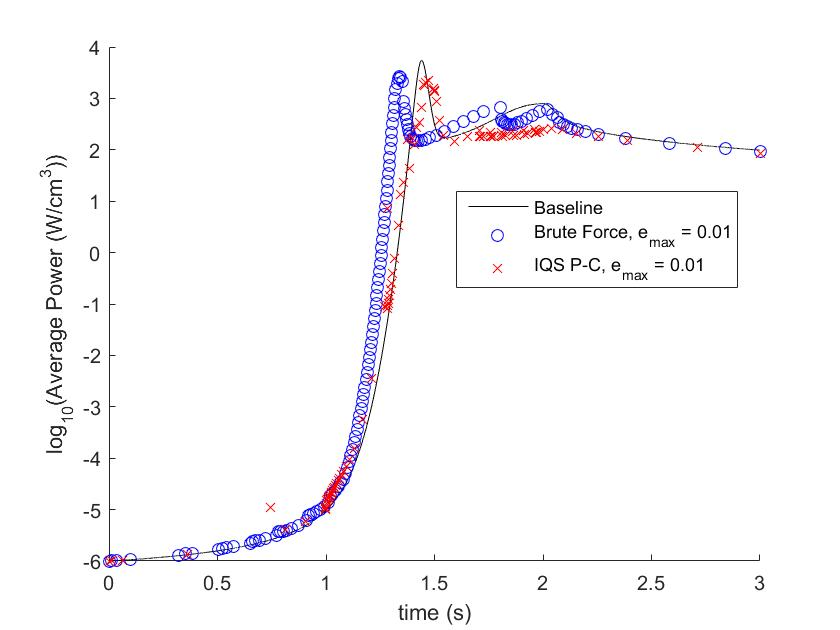
\includegraphics[width=0.5\textwidth]{lra_power_profile.jpg}
%\caption{Power level comarison of LRA benchmark between IQS and Brute Force using $e_{max} = 0.01$}
%\label{fig:LRA_plots}
%\end{center}
%\end{figure}
%
%\begin{table}[!htbp]
%\begin{center}
%\resizebox{0.48\textwidth}{!}{
%\begin{tabular}{|l|l|l|l|l|l|l|l|}
%\hline
%  &  & \multicolumn{3}{|c|}{Brute Force} & \multicolumn{3}{|c|}{IQS P-C} \\
%\hline
%Test & $e_{max}$ & Error & Steps & Solves & Error & Steps & Solves \\
%\hline
%1 &	0.01    &	3.5555e-05 &	145  &	735  &	0.00263068 &	105 &	616  \\
%2 &	0.005   &	4.0364e-05 &	266  &	948  &	0.00160486 &	157 &	814  \\
%3 &	0.001   &	0.00294822 &	585  &	2046 &	1.7527e-05 &	218 &	1062  \\
%4 &	0.0005  &	0.00099778 &	833  &	2908 &	1.4185e-05 &	480 &	2038  \\
%5 &	0.0001  &	0.00019510 &	1793 &	6155 &	6.2903e-06 &	434 &	1458  \\
%6 &	5.0e-05 &	0.00018372 &	2485 &	8511 &	1.5247e-06 &	542 &	1719  \\
%\hline
%
%\end{tabular}}
%\end{center}
%\caption{LRA step doubling results}
%\label{tab:LRAdt2}
%\end{table}

%%%%%%%%%%%%%%%%%%%%%%%%%%%%%%%%%%%%%%%%%%%%%%%%%%%%%%%%%%%%%%%%%%%%%%%%%%%%%%%%
\section{Conclusions}

The purpose of this paper was to show IQS's performance with step doubling time adaptation.  The TWIGL benchmark was used to quantify the method's performance.  The results from the TWIGL example shows significant improvement from the traditional brute force method.  This improvement was anticipated because the shape for TWIGL changes very little through the transient, so the PRKE in IQS does most of the work.  In conclusion, IQS shows impressive performance for complex neutronics problems with time adaptation.  However, to rigorously test IQS, more complex problems including TREAT models and transport problems need to be applied.

%%%%%%%%%%%%%%%%%%%%%%%%%%%%%%%%%%%%%%%%%%%%%%%%%%%%%%%%%%%%%%%%%%%%%%%%%%%%%%%%
%\appendix
%\section{Appendix}

%%%%%%%%%%%%%%%%%%%%%%%%%%%%%%%%%%%%%%%%%%%%%%%%%%%%%%%%%%%%%%%%%%%%%%%%%%%%%%%%
\section{Acknowledgments}

This work was supported by the Department of Energy and Idaho National Laboratory.  Special thanks to Mark Dehart, Yaqi Wang, NEAMS, and the Moose/Rattlesnake team at INL.

%%%%%%%%%%%%%%%%%%%%%%%%%%%%%%%%%%%%%%%%%%%%%%%%%%%%%%%%%%%%%%%%%%%%%%%%%%%%%%%%
\bibliographystyle{ans}
\bibliography{references_IQS}
\end{document}

